%\documentclass[10pt]{article}
%%\input{../../common/1021_header.tex}
%\input{../../common/header_old.tex}
%\usepackage{tikz, wasysym, framed}
%
%\newcommand{\ihat}{\boldsymbol{\hat{\textbf{\i}}}}
%\newcommand{\jhat}{\boldsymbol{\hat{\textbf{\j}}}}
%\newcommand{\khat}{\boldsymbol{\hat{\textbf{k}}}}
%
%\let\oldvec\vec
%\renewcommand{\vec}[1]{\oldvec{\mathbf{#1}}}
%
%\newcommand{\uhat}{\boldsymbol{\hat{\textbf{u}}}}
%\newcommand{\grad}{\vec{\nabla}}
%\newcommand{\<}{\left\langle}
%\renewcommand{\>}{\right\rangle}
%
%
%\begin{document}
% Instructions to change to html version:
% Comment out:
%  minipage, multicols,columnbreak, mathbf, hrule
% Replace all:% %\begin{minipage}% %%%\end{minipage} %%%%%%\begin{mulicols}  %%%%%%\end{mulicols}  %%%%%\columnbreak % %%%%%\begin{framed} %%%%%\endframed} %%%%%\hrule
% Search for \mathbf
% Replace \\] with \[ and \) with \(
% Enclose graphics in figure environments and add captions
% Re-tag \df environments as sections, subsections, etc.
% Command Line Code to Create html version:
%First: pdflatex -shell-escape filename.tex                                   
%Second, for each figure: inkscape "filename-figure1.pdf" -o "filename-figure1.png"
% Third: htlatex filename.tex "ht5mjlatex.cfg, charset=utf-8" " -cunihtf -utf8"


\documentclass[10pt]{article}

%\usepackage{tikz, pgf,pgfplots,wasysym,array}
%\usepackage{wasysym,array}

\usepackage{amsmath,amssymb}

\ifdefined\HCode
  \def\pgfsysdriver{pgfsys-tex4ht-updated.def}
\fi 
%\ifdefined\HCode
%  \def\pgfsysdriver{pgfsys-dvisvgm4ht.def}
%\fi 
\usepackage{tikz}
\usetikzlibrary{calc,decorations.markings,arrows}
\usepackage{pgfplots}

\pgfplotsset{compat=1.12}
\usepackage{myexternalize}
\usetikzlibrary{calc,decorations.markings,arrows}
\usepackage{framed}
\usepackage[none]{hyphenat}

\input{../../../common/1336_header_test.tex}

\newcommand{\ihat}{\boldsymbol{\hat{\textbf{\i}}}}
\newcommand{\jhat}{\boldsymbol{\hat{\textbf{\j}}}}
\newcommand{\khat}{\boldsymbol{\hat{\textbf{k}}}}

%\let\oldvec\vec
%\renewcommand{\vec}[1]{\oldvec{\mathbf{#1}}}

\newcommand{\uhat}{\boldsymbol{\hat{\textbf{u}}}}
\newcommand{\grad}{\vec{\nabla}}
\newcommand{\<}{\left\langle}
\renewcommand{\>}{\right\rangle}


\begin{document}


\renewcommand{\myTitle}{MATH 2330: Multivariable Calculus}

\renewcommand{\mySubTitle}{4.6: Directional Derivatives \& The Gradient}% - Part 2}
%~\hfill Name: \underline{~~~~~~~~~~~~~~~~~~~~~~~~~~~~~~~~~~~~~~~~~~~~~~~}

\lectTitle{\vspace*{-.5in}\myTitle}{\vspace*{.1in}\mySubTitle \vspace*{-.25in}}

%

%\vspace*{-.5in}
\section*{Section 4.6 -  Directional Derivatives \& The Gradient:}

\hspace*{-.8in}%\begin{minipage}{1.25\textwidth}
%\begin{framed}

\subsection*{Definitions \& Terminology:}
%\begin{multicols}{2}
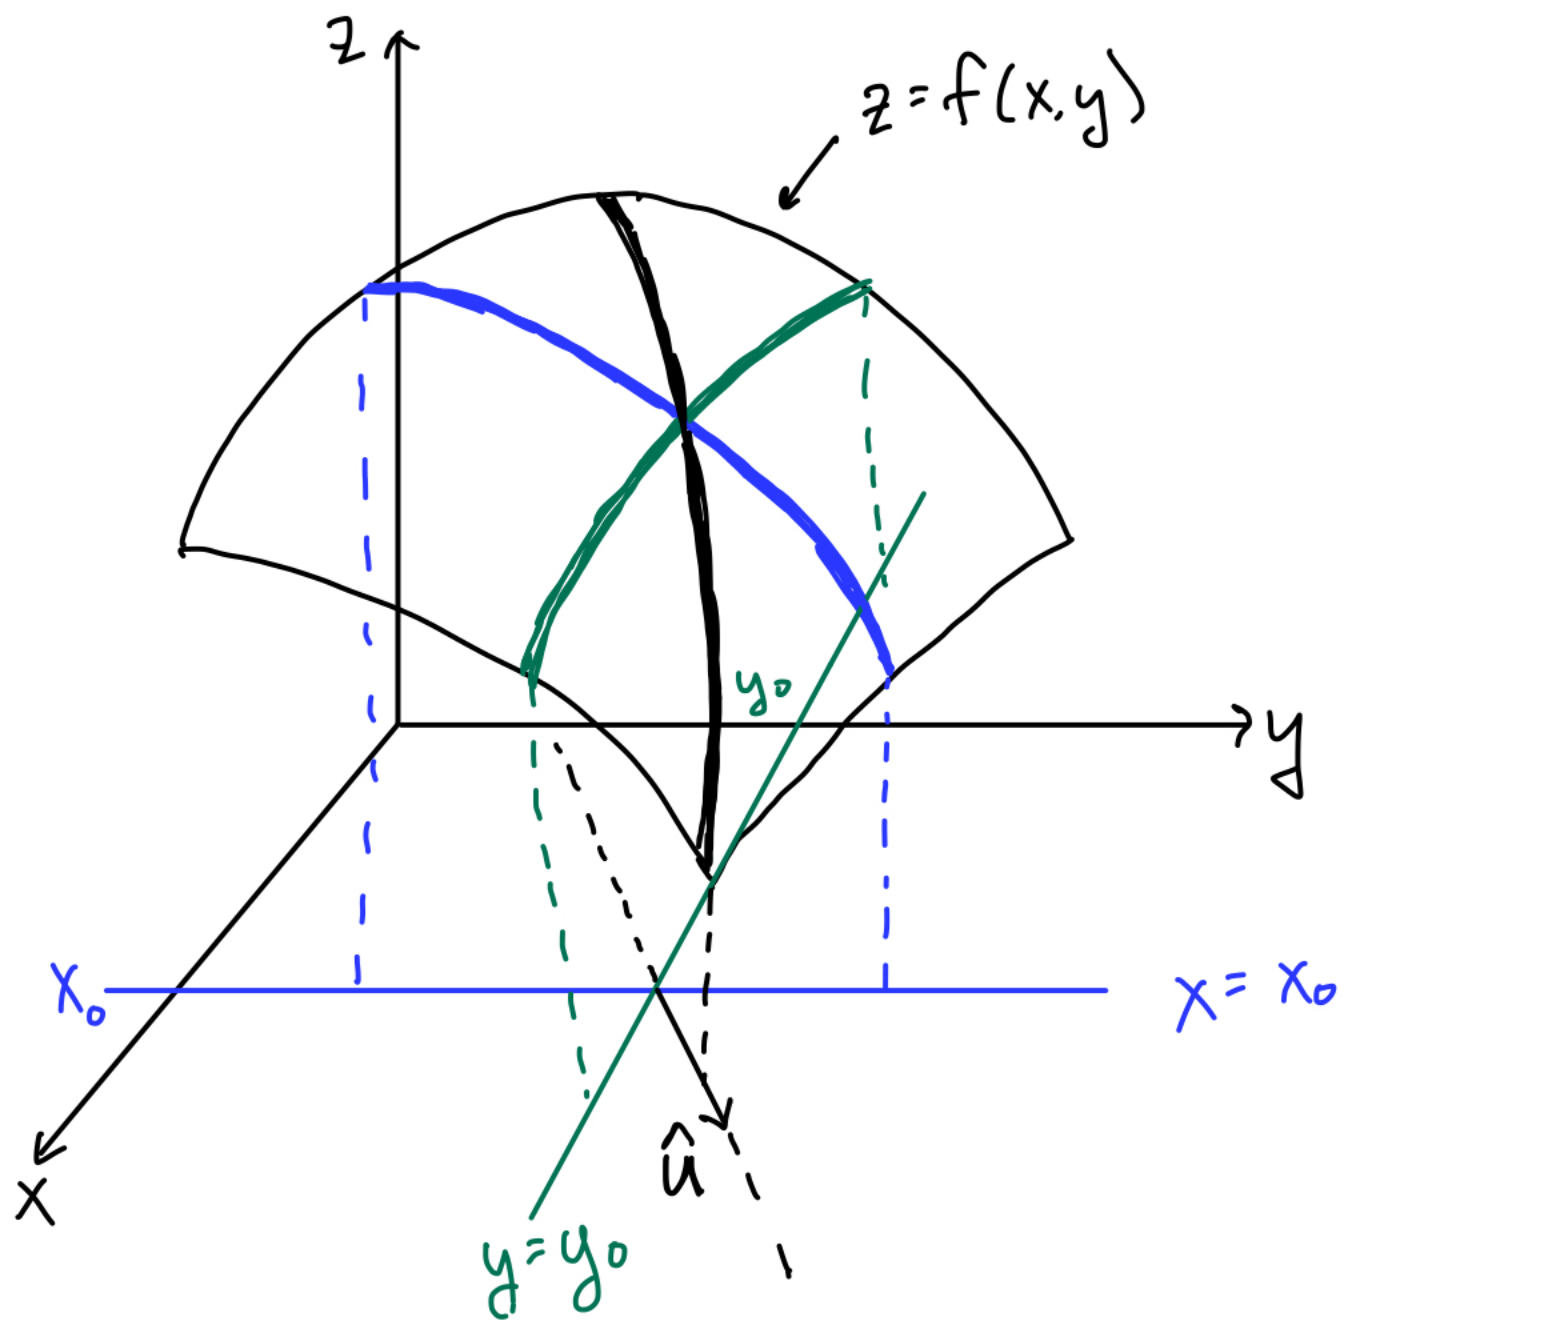
\includegraphics[width=\columnwidth]{Directional-Derivative.png}



\textbf{Directional Derivative:}~\\

The \textbf{Directional Derivative} in the \(\uhat\) direction calculates the slope of the surface in the direction of the vector \(\uhat\).\\

 If \(f\) is a differentiable function of \(x\) and \(y\), then \(f\) has a directional derivative in the direction of any \textbf{unit vector} \(\uhat = \<a,b\>\) that can be calculated using:
\[
D_u f(x,y) = f_x(x,y) a + f_y(x,y) b=  \grad f \cdot \uhat\\
\]


\vspace*{.2in}

\textbf{The Gradient:}
\[
\grad f = \<f_x,f_y\>
\]


%\end{multicols}


%\end{framed}

%\end{minipage}

\textbf{Discussion:} Geometric Implications of \(D_u f(x,y) = \grad f \cdot \uhat\).

\vfill

\pagebreak

\begin{enumerate}[{Example} 1: ]
%\addtocounter{enumi}{1}
\item Find the directional derivative of \(f(x,y)=\ln(x^2+y^3)\) at \((1,-3)\) in the direction of \(\vec{v} = 2\ihat-3\jhat\).\\

\hspace*{-.25in}%\begin{minipage}{.5\textwidth}

\underline{\textbf{Questions about the solution from the Video? }}

\begin{eqnarray*}
D_v f &=& \grad f(1,-3) \cdot \boldsymbol{\hat{\textbf{v}}}\\~\\
&=& \left. \<\frac{2x}{x^2+y^3}\ , \frac{3y^2}{x^2+y^3}\>\right|_{(1,-3)} \cdot \< \frac{2}{\sqrt{13}}\ ,-\ \frac{3}{\sqrt{13}}\>\\~\\
&=& \< -\ \frac{2}{26}\ , -\ \frac{27}{26}\> \cdot \< \frac{2}{\sqrt{13}}\ ,-\ \frac{3}{\sqrt{13}}\>\\`\\
&=& \left(-\ \frac{2}{26}\right)\left(\frac{2}{\sqrt{13}}\right) + \left(-\ \frac{27}{26} \right) \left( -\ \frac{3}{\sqrt{13}}\right)\\~\\
&=& \frac{77}{26\sqrt{13}} \ \ \ = \ \frac{77\sqrt{13}}{338}
\end{eqnarray*}


%\end{minipage}

\vspace*{.2in}

\item In what direction is the function \(f(x,y) = x e^{2y-x}\) increasing most rapidly at \((2,1)\), and what is the maximum rate of increase?
\vfill

\item \textbf{Hiker Problem:}\\
A hiker is walking on a mountain path when it begins to rain.  If the height of the mountain is modeled by the equation \(z= f(x,y)=1-3x^2-\frac{5}{2}y^2\), where \((x,y,z)\) are measured in miles, and the rain begins when the hiker is at the point \(\left(\frac{1}{4},\frac{-1}{2},\frac{3}{16}\right)\), in what direction should she head to descend the mountainside most rapidly?\\

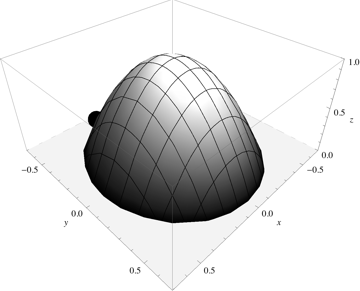
\includegraphics[width=.4\textwidth]{problemPlot.png}
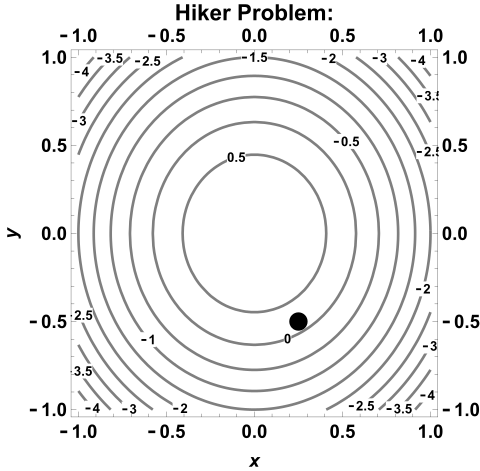
\includegraphics[width=.4\textwidth]{hikeContour.png}

\vfill

\pagebreak

\item \textbf{Example from Marsden, Tromba, \& Weinstein, ``Basic Multivariable Calculus''}\\~\\
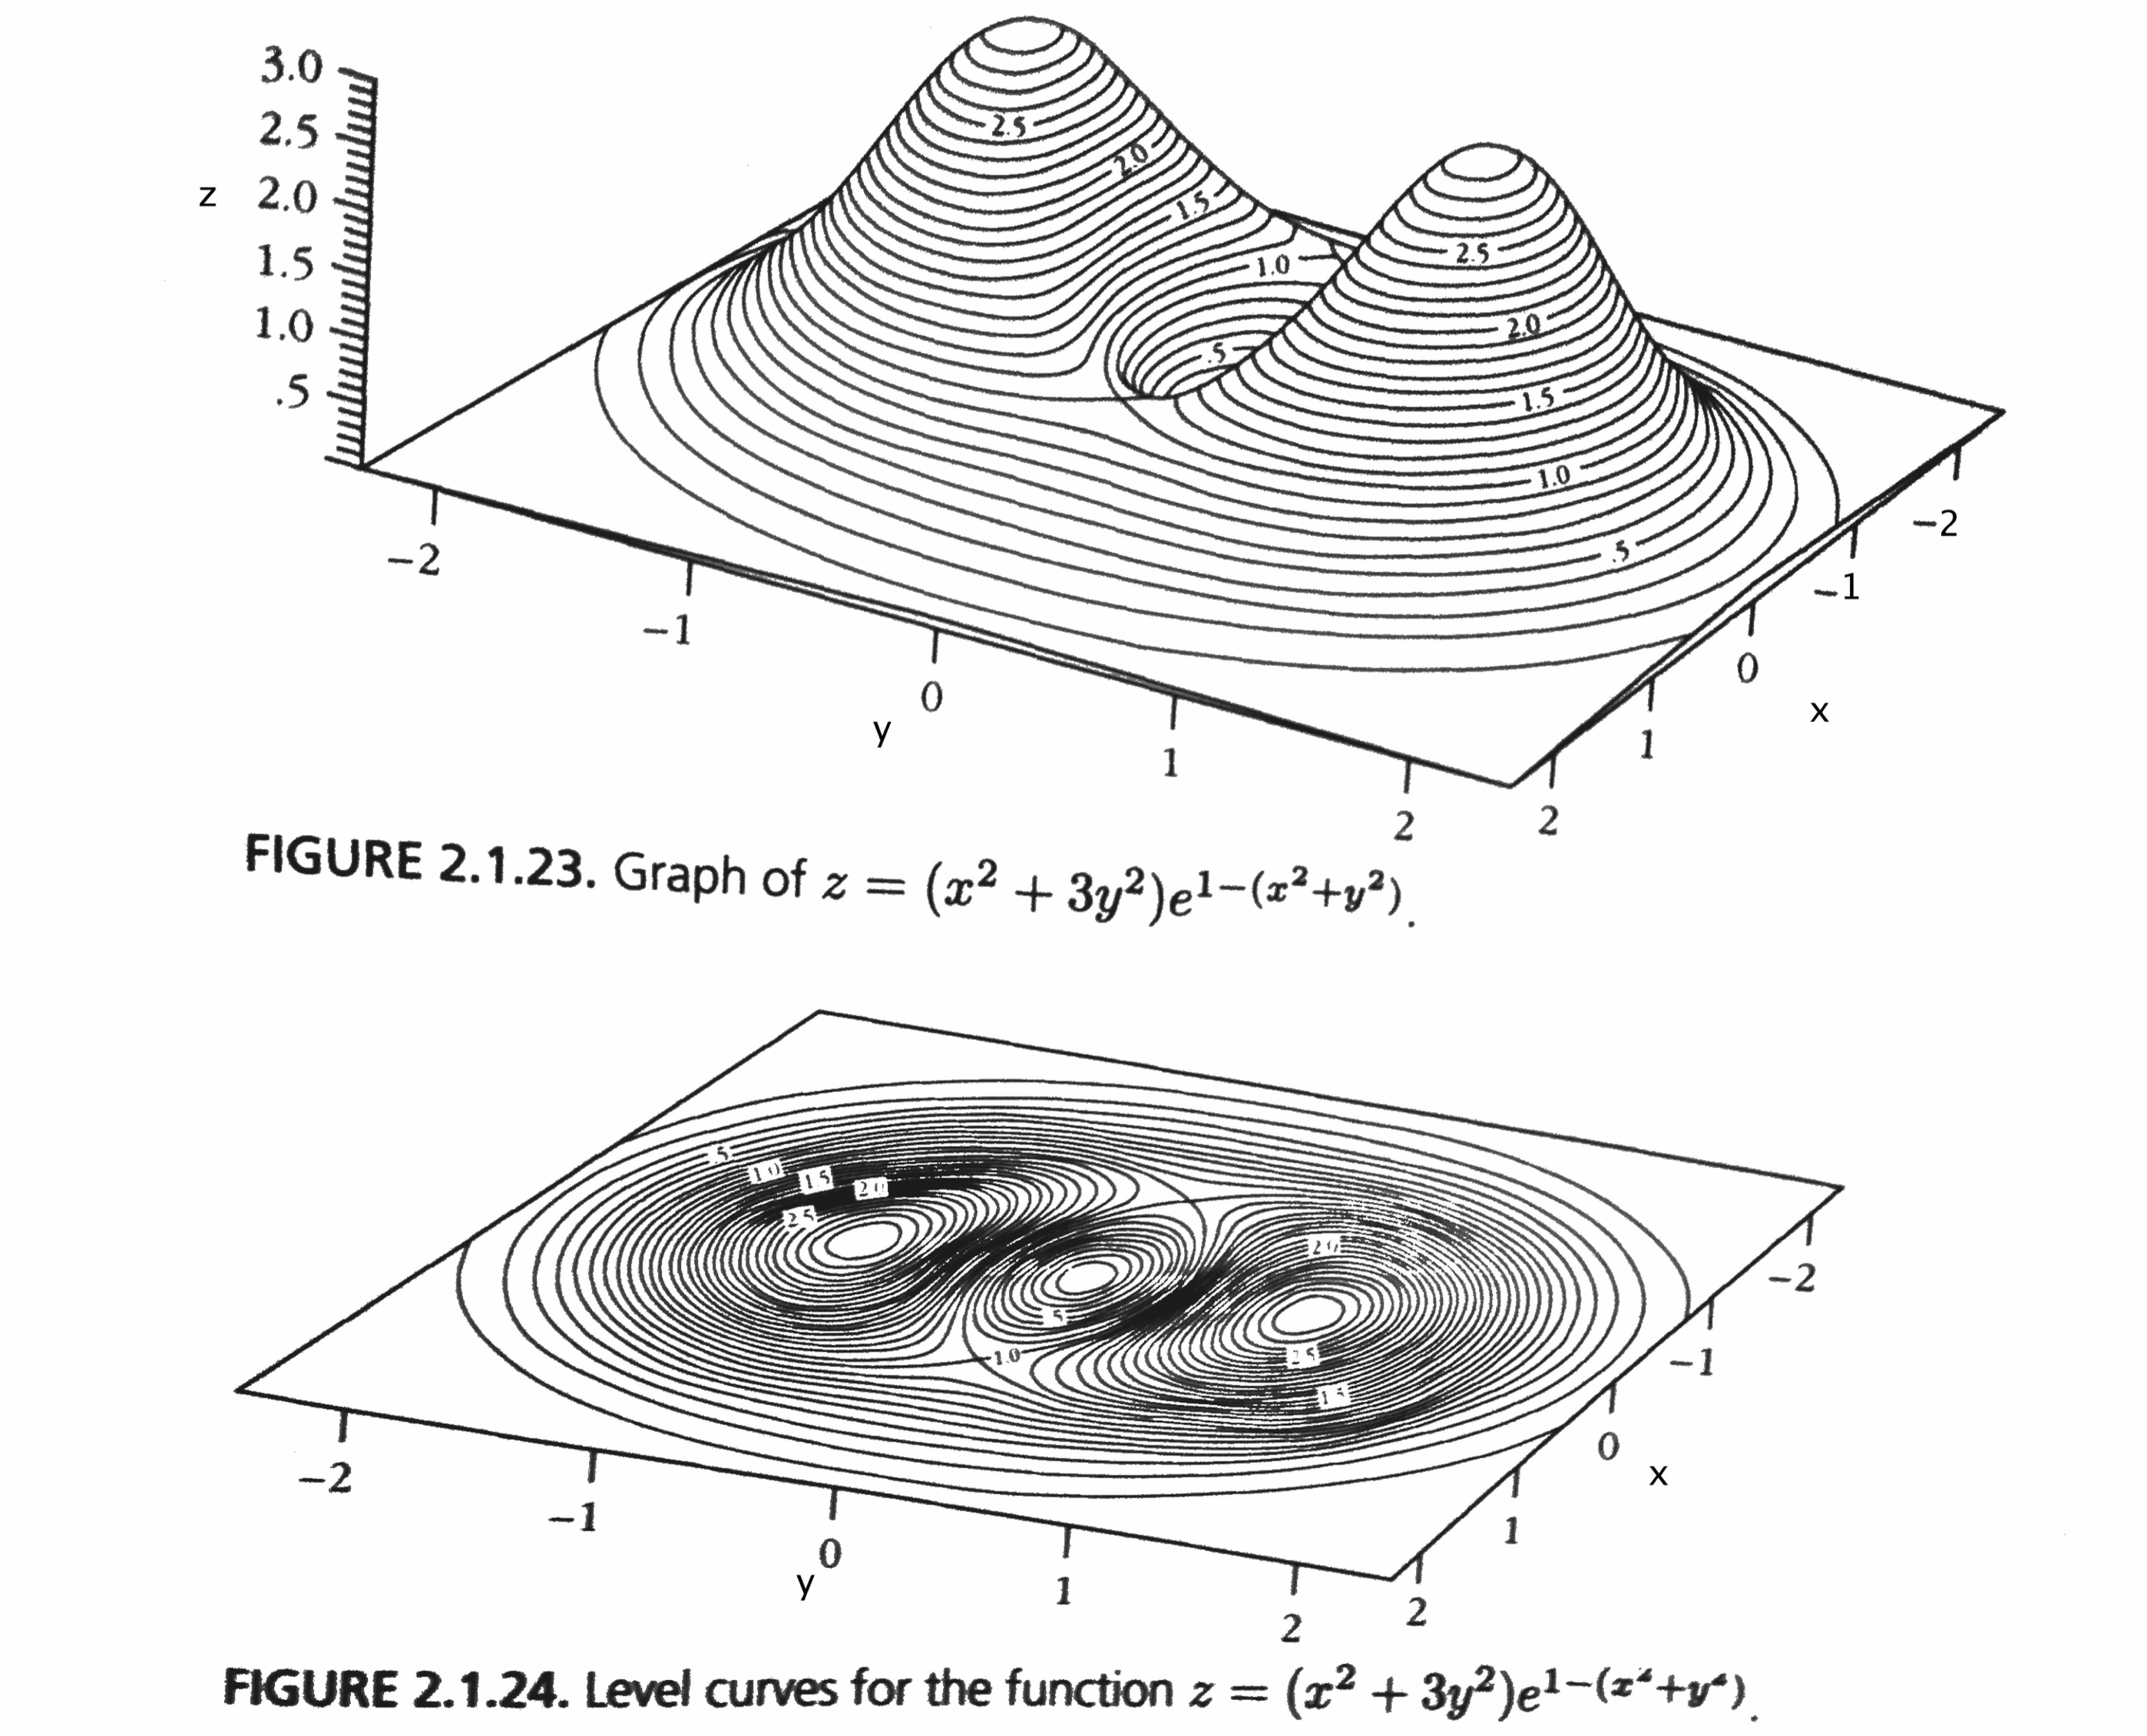
\includegraphics[width=.8\textwidth]{Surface3.png}\\

\vspace*{.5in}
\hspace*{-1.5in}
%\begin{minipage}{.5\textwidth}
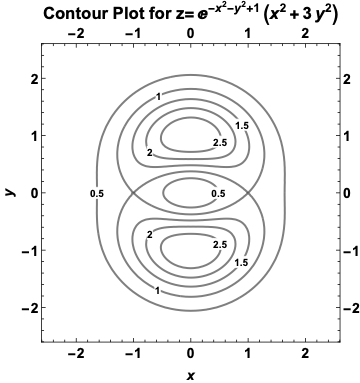
\includegraphics[width=\textwidth]{SurfContour.png}
%\end{minipage} \hspace*{.2in}
%\begin{minipage}{.6\textwidth}
Answer the following questions about the surface\\ \(z=f(x,y)\), shown in the figures on this page, at the point \((1.2,-1)\):
\begin{itemize}
\item Which way should the gradient vector point?
\item Is \(f_x > 0\)?
\item In which direction would water flow?
\item Is \(D_u f\) positive, negative, or zero for \(\vec{u} = \langle 1,1\rangle\)?
\item Find a direction in which \(D_u f \approx 0\).
\end{itemize}
Now, pick some other point, and answer the questions again!
%\end{minipage}
\end{enumerate}



\end{document}

